\documentclass[UTF8]{ctexrep}
% package
% page size setting
\usepackage{geometry}

% layout
\usepackage{multicol}

% using [H] to ban the float of algorithm, figure and so on.
\usepackage{float}

% insert pdf page
\usepackage{pdfpages}

% color
\usepackage{xcolor}

% figure
\usepackage{graphicx}
\usepackage[]{subfig}

% table
\usepackage{multirow}
\usepackage{array}

% math
\usepackage{amsmath}
\usepackage{amssymb}
% some custom math symbols
\newcommand{\vect}[1]{\boldsymbol{#1}} % vector
\newcommand{\mat}[1]{\mathbf{#1}}      % matrix
\newcommand{\tensor}[1]{\mathsf{#1}}   % tensor
\newcommand{\set}[1]{\mathbb{#1}}      % set
\newcommand{\T}{\mathrm{T}}        % transposition
\everymath{\displaystyle}              % block style for inline math


% code
%% float of algorithm
\usepackage{algorithm}
%% body of algorithm
\usepackage{algorithmic}
%% custom setting for algorithmic
\renewcommand{\algorithmicrequire}{\textbf{Input:}}
\renewcommand{\algorithmicensure}{\textbf{Output:}}
%% highlight
\usepackage{minted}

\usepackage{multicol}

% reference
\usepackage[]{hyperref}
\hypersetup{
    colorlinks=true,
}

% URL
\usepackage{url}
\usepackage{lipsum}

\geometry{
    a4paper,
    left=15mm,
    right=15mm,
    top=15mm,
    bottom=15mm,
    marginparwidth=15mm
}


\renewcommand{\equationautorefname}{公式}
\renewcommand{\figureautorefname}{图}
\renewcommand{\tableautorefname}{表}
\newcommand{\subfigureautorefname}{图}
\newcommand{\algorithmautorefname}{算法}
% \usepackage{abstract}

% \renewcommand\refname{参考文献}
\usepackage[backend=biber,style=gb7714-2015]{biblatex}
\addbibresource{ref.bib}


%% custom refname for algorithm
\renewcommand{\equationautorefname}{式}
\renewcommand{\figureautorefname}{图}
\renewcommand{\tableautorefname}{表}
\renewcommand{\subfigureautorefname}{子图}
\renewcommand{\algorithmautorefname}{算法}
%% Custom refname for step of algorithm
\makeatletter
\newcommand{\ALC@uniqueautorefname}{步}
\makeatother
% \newcommand{\upcite}[1]{\textsuperscript{\cite{#1}}}

\title{\LaTeX 中文报告模板}
\author{姓名}
\date{\today}

\begin{document}

\pagestyle{plain}
\setcounter{page}{1}
\pagenumbering{Roman}
\maketitle
{
    \hypersetup{linkcolor=black}
    \tableofcontents
    \newpage
}
\setcounter{page}{1}
\pagenumbering{arabic}
\pagestyle{headings}

\chapter{\LaTeX}
\label{chapter:example}

\section{文本}

\begin{enumerate}
    \item 正常
    \item \textbf{加粗}
    \item \textit{斜体}
    % \item \sout{删除线}
    % \item \xout{italic delete line}
    % \item \uwave{波浪线}
    \item \underline{下划线}
    % \item \uline{underline}
    % \item \uuline{double underline}
    % \item \dashuline{dash underline}
    % \item \dotuline{dot underline}
    \item \colorbox{yellow}{highlight}
\end{enumerate}

\section{图片}

\subsection{单图}

\begin{figure}[H]
    \centering
    
\includegraphics[width=0.7\textwidth]{./img/logo.png}
    \caption{SCUT 的 Logo}
    \label{fig:logo}
\end{figure}

\subsection{子图}

\begin{figure}[H]
    \centering
    \subfloat[子图 1\label{fig:subfig-1}]{
        
\includegraphics[width=0.12\textwidth]{./img/logo-short.png}
    }
    \hspace{1em}
    \subfloat[子图 2\label{fig:subfig-2}]{
        
\includegraphics[width=0.5\textwidth]{./img/logo.png}
    }
    ~\\
    \subfloat[子图 3\label{fig:subfig-3}]{
        
\includegraphics[width=0.5\textwidth]{./img/logo.png}
    }
    \hspace{1em}
    \subfloat[子图 4\label{fig:subfig-4}]{
        
\includegraphics[width=0.12\textwidth]{./img/logo-short.png}
    }
    \caption{子图}
    \label{fig:subfig}
\end{figure}

\section{表}
\begin{table}[H]
    \centering
    \caption{参数值}
    \label{tb:paramter}
    \begin{tabular}{c|c}
    \hline
    Parameter & Value \\ \hline
    $\alpha$  & 1     \\ \hline
    $\beta$   & 1     \\ \hline
\end{tabular}
\end{table}
\begin{table}[H]
    \centering
    \caption{参数值}
    \label{tb:figure}
    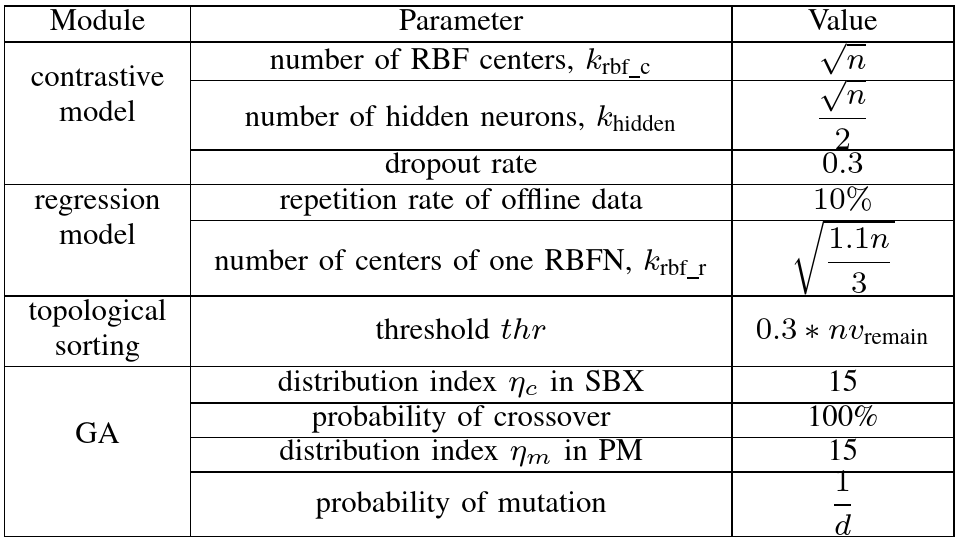
\includegraphics[width=0.65\textwidth]{./table/figure.png}
\end{table}
有时候太懒了,直接截图,把图片扔到 table 环境,例如上边的表。

\section{伪代码}
\begin{center}
    \begin{minipage}{0.55\textwidth}
        \begin{algorithm}[H]
            \centering
            \caption{KahnAlgorithm}
            \label{algo:kaha}
            \begin{algorithmic}[1]
    \REQUIRE Graph $G(\mathbb{V}, \mathbb{E})$
    \ENSURE Sequence $L$
    \STATE $L \leftarrow$ an empty sequence
    \STATE $Q \leftarrow$ the vertices whose indegree is zero
    \WHILE{$Q$ is not empty}
        \STATE $u \leftarrow$ remove the top node of $Q$
        \STATE add $u$ to $L$
        \FOR{each node $v$ with an edge $e$ from $u$ to $v$}
            \STATE remove edge $e$ from graph $G$
            \IF{indegree of $v$ is $0$}
                \STATE push $v$ to $Q$
            \ENDIF
        \ENDFOR
    \ENDWHILE
    \RETURN $L$
\end{algorithmic}
        \end{algorithm}
    \end{minipage}
\end{center}

\begin{center}
    \begin{minipage}{0.55\textwidth}
        \begin{algorithm}[H]
            \scriptsize
            \caption{框架}
            \label{aglo:figure}
            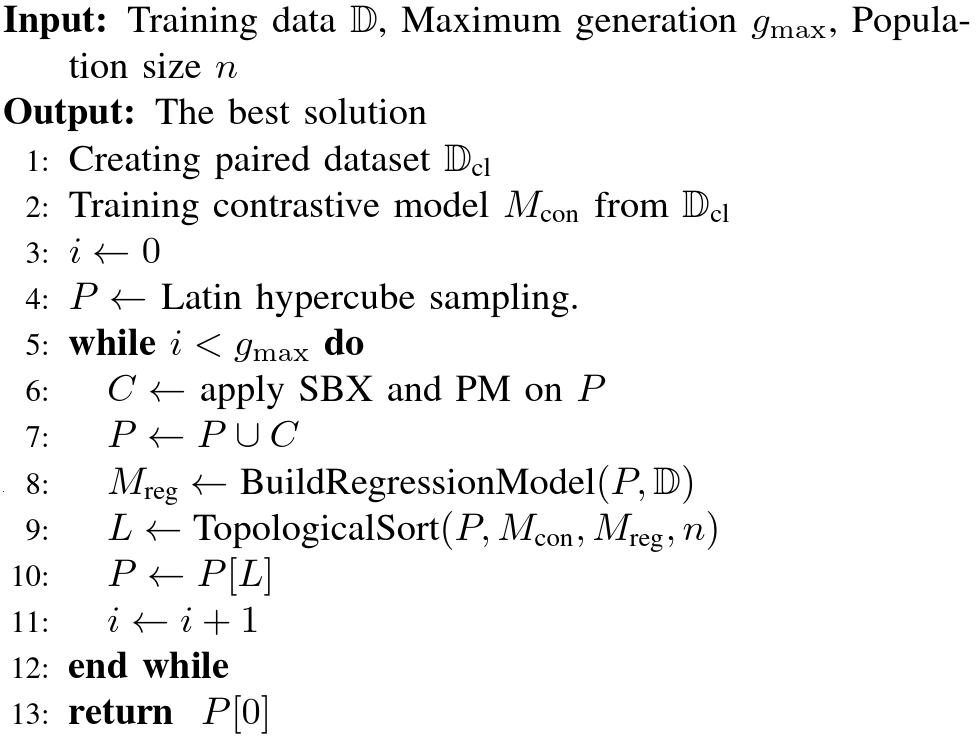
\includegraphics[width=\textwidth]{./algo/figure.png}
        \end{algorithm}
    \end{minipage}
\end{center}
有时候太懒了,直接截图,把图片扔到 algorithm 环境,例如上边的算法。

\section{高亮}

\inputminted[linenos]{cpp}{./code/quicksort.cpp}

\section{多栏}
\begin{multicols}{2}
    \lipsum[1-3]
\end{multicols}

\section{数学}

Interline Formula:
\begin{equation}
    \label{eq:example}
    a_n = a_{n-1} + 1
\end{equation}

行内公式:
这是一个简单的等差数列公式 $a_n = a_{n-1} + 1$ 。

\section{Ref}
\begin{itemize}
    \item 图片: \autoref{fig:logo}
    \item 子图: \autoref{fig:subfig-1}
    \item 表: \autoref{tb:paramter}
    \item 伪代码: \autoref{algo:kaha}
    \item 公式: \autoref{eq:example}
    \item 章: \autoref{chapter:example}
    \item 论文: \cite{he2016deep}
    \item URL 1: \href{https://baidu.com}{baidu}
    \item URL 2: \url{https://baidu.com}
\end{itemize}


\printbibliography[title={参考文献}]

\end{document}
